% !TEX root =  main.tex

Nella presente sezione vengono discusse le scelte implementative per la
realizzazione di un sistema come quello descritto nella
sezione~\ref{sec:components}. Le componenti vengono infatti declinate nel caso
specifico di una rete (Jolella) che presenterà differenze (anche se piccole) per
ogni gruppo di studenti coinvolto nella realizzazione di questo progetto.

\subsection{La rete Jolella}
\label{subsec:jolella}

Jolella, ispirata al programma Gnutella~\cite{gnutella}, è una rete
decentralizzata per la condivisione di files tra nodi della rete stessa (anche
detta \textit{P2P})~\footnote{Creato nel 2000, è stato uno dei primi protocolli
 di condivisione di files su una rete decentralizzata peer-to-peer.}.

\paragraph{Architettura di Jolella.} La scelta dell'architettura della rete non è
vincolata, il progetto potrà infatti essere svolto seguendo una delle tre
strategie proposte. Viene invece richiesta coerenza nelle scelte implementative
derivanti dall'architettura selezionata, ed una concisa documentazione sulle
motivazioni che hanno portato a tale scelta.

\subsubsection{Obiettivi e Problemi dei sistemi P2P}

Esistono motivazioni specifiche per cui si è scelto il sistema P2P nella
realizzazione del progetto proposto. Alcune risiedono nelle caratteristiche del
sistema stesso, altre, legate ad esigenze didattiche, mirano a mettere in luce
il livello di apprendimento raggiunto su alcuni concetti teorici specifici (ad
esempio quelli relativi alla \textbf{gestione della concorrenza}).

Tra le caratteristiche del sistema alcune sono interessanti rispetto alle
soluzioni ``centralizzate''. Queste sono l'aumento di scalabilità (la creazione
di un peer e del milionesimo peer è uguale); l'interoperabilità e la possibilità
di aggregazione delle risorse; l'autonomia ed il dinamismo (se un peer si
disconette, la rete non subisce modifiche).

Alcune limitazioni sono imposte sulla strategia di realizzazione del progetto
per innescare l'esigenza di risoluzione del problema proposto e consolidare così
i concetti teorici. Le criticità dei sistemi P2P da considerare, sono (in ordine
sparso): la \textbf{sicurezza e consistenza delle comunicazioni}, la
\textbf{disuguglianza tra nodi} e \textbf{l'elevato dinamismo o instabilità
 della rete}. Una particolare attenzione va riservata a questi aspetti, la cui
risoluzione costituisce il fulcro stesso del progetto.

\paragraph{Altri vincoli e limitazioni.} Di seguito alcuni vincoli che, per
semplicità, vengono imposti sul sistema:

\begin{itemize}

 \item assumiamo che la ricerca per keyword, sia effettuata sui
       nomi dei file, e che questi corrispondano con l'effettivo contenuto
       (non sono \textit{fake files}).

 \item assumiamo che la rete sia una rete \textbf{non strutturata}, cioè
       organizzata come un \textbf{grafo random} e dove non esistono vincoli sul
       posizionamento dei nodi rispetto alla topologia del grafo. In questa
       configurazione l'aggiunta o la rimozione del nodo non comporta la
       riorganizzazione della rete. Per delucidazioni sui grafi consiglio i lucidi presenti in~\cite{grafi}, alla voce ``Grafi''.

 \item in caso di sistemi ad architettura puramente decentralizzata, e quindi
       con ricerca flood-based, si richiede l'utilizzo di un  ID per ogni query, così
       da controllare che questa non sia già stata risolta dal nodo  ricevente.

\end{itemize}

Non esistono vincoli di alcun tipo sull'uso di linguaggi (supportati da Jolie)
per la creazione di servizi. L'unica limitazione è sull'uso di Jolie per
implemetare la comunicazione tra i servizi creati.

Un esempio di servizio creato in \textit{Java} (attualmente le tecnologie
supportate da Jolie sono Java e Javascript) può essere trovato in
\href{https://github.com/szingaro/jolie-file-worker}{questa \textit{repository}
 di GitHub}.

\subsection{Il Jeer}
\label{subsec:jeer}

Un peer della rete Jolella (che, per disambiguità, chiameremo \textbf{Jeer}) si
può occupare sia delle operazioni di gestione della rete, sia delle funzionalità
del singolo peer (descritte entrambe nella sezione~\ref{subsec:p2p}).

In Gnutella, i peer offrono una operazione di \textbf{discovery} che permette ad
un nodo che conosce l'indirizzo di un altro nodo, di accedere alle liste di nodi
connessi. Per la ricerca, il  nodo utilizza un algoritmo flood-based di tipo
\textit{breadth-first} (BFS).

\begin{figure}[H]
 \centering
 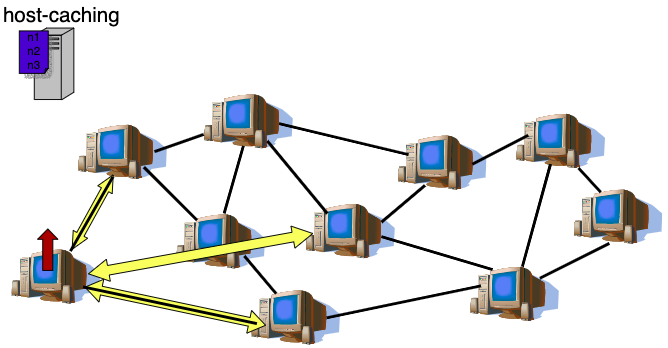
\includegraphics[width=0.75\textwidth]{gnutella}
 \caption{Un peer può rifiutare una richiesta di connessione, ad esempio perché ha raggiunto un numero massimo di connessioni ammesse.}
\end{figure}

\subsection{Monitorare Jolella ed i Jeer}

Abbiamo bisogno di un sistema di feedback per il monitoraggio della rete, sia in
fase di \textit{debugging}, che durante la manutenzione del sistema. Inoltre,
durante la prova orale, sarò necessario per il controllo della corretta
implementazione del soluzioni proposte dal gruppo. Il monitor può essere visto
come una console di \textit{logging}, dove è possibile visualizzare lo storico
della rete. Esso può essere stampato a video oppure su un file. Un esempio di
output del monitor della rete potrebbe consistere nel semplice elenco numerato
riportato in basso, \textbf{la numerazione è obbligatoria}.

\begin{verbatim}
1. La rete Jolella è attiva!
2. Il Jeer <id_jeer> ora partecipa alla rete.
3. Il Jeer <id_jeer> ha pubblicato il Jile <id_jile>
\end{verbatim}
